% !TEX root = main.tex

本课程采用书目Avi Silberschatz, Henry F. Korth, S. Sudarshan, \emph{Database System Concepts (6th ed)}\footnote{\url{http://www.db-book.com}}。

\section{数据库系统概述} % Chap 1, 2
\subsection{高层概述}
早期的数据库直接建立在文件系统上,但这会导致:
\begin{itemize}
	\item 数据冗余与不一致
	\item 访问数据非常麻烦
	\item 数据孤立:数据分散在不同文件中,文件又有不同格式
	\item 完整性问题:难以添加限制(如年龄为非负整数)
	\item 原子性问题:要么全部发生要不根本不发生
	\item 多用户的并发访问
	\item 安全性问题:权限
\end{itemize}

数据抽象包括下述三级
\begin{figure}[H]
\centering
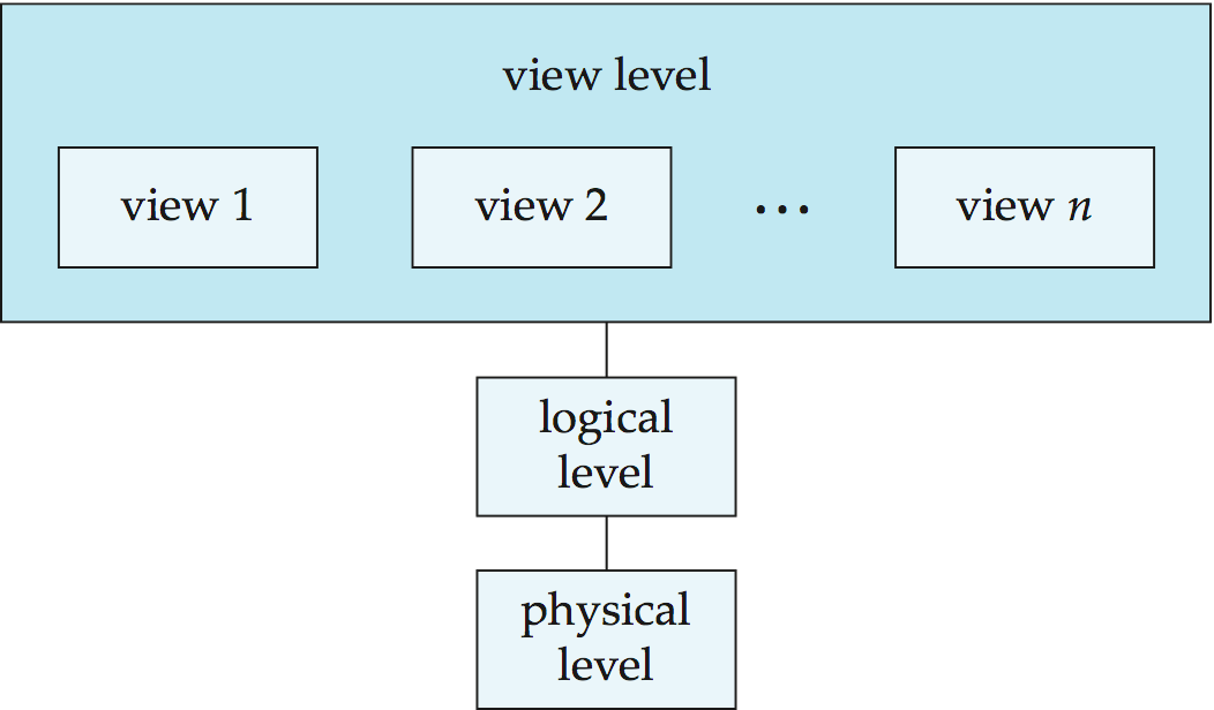
\includegraphics[width=0.5\linewidth]{fig/view_of_data.png}
\end{figure}
\begin{itemize}
	\item 视图层:屏蔽数据类型细节的一组应用程序,同时提供了访问权限
	\item 逻辑层:通过类型定义进行描述,同时记录类型之间的相互关系
	\item 物理层:存储块、物理组织
\end{itemize}

查询过程:解释编译+求值(evaluation)

数据模型:关系模型、实体-联系模型(ER)、基于对象的数据模型、半结构化数据模型(XML)

\subsection{数据库语言}
\begin{itemize}
\item 数据操纵语言(Data Manipulation Language, DML)
\item 数据定义语言(Data Definition Language, DDL):DDL的输出放在数据字典中,数据字典包含元数据(metadata),需要满足一致性约束
\begin{itemize}
	\item 域约束:如整型、字符型等
	\item 参照完整性(referential integrity):一个关系中给定属性集上的取值也在另一关系的某一属性集的取值中出现,如
	course记录中的dept\_name必须出现在department关系dept\_name属性中
	\item 断言(assertion):域约束和参照完整性只是断言的特殊形式,如“每一学期每一个系必须至少开设5门课程”
	\item 权限(authorization)
\end{itemize}
\end{itemize}

\subsection{关系型数据库}
\subsubsection{结构}
每一个表(table)都是一个\underline{关系}(relation),纵向为\underline{属性}(attributes/columns),横向为\underline{元组}(tuples/rows)。
一组特定的行称为关系\underline{实例}(instance)。
\begin{center}
\begin{tabular}{|c|c|c|}\hline
\textbf{ID} & \textbf{name} & \textbf{dept\_name}\\\hline
12345 & Chen & CS\\
10001 & Bob & Biology\\
10101 & Alice & Physics\\\hline
\end{tabular}
\end{center}
注意关系都是无序的,元组可以以任意顺序存储。

数据库模式(schema)是数据库的逻辑设计,如\verb'instructor(ID,name,dept_name,salary)'(可以理解为是一个抽象);
数据库实例(instance)则是给定时刻数据库中数据的一个快照,与具体数据相关。

关系对应着程序设计语言中变量的概念,而关系模式(relation schema)的概念对应于程序设计语言中类型定义的概念。
关系模式一定是\verb'<name>(<attr1>,...,<attrn>)'的形式。

\subsubsection{码}
一个元组的属性值必须是能\textbf{唯一}区分元组的,即一个关系中没有两个元组在所有属性上取值都相同。
\begin{itemize}
\item 超码(superkey):\textbf{一个或多个}属性的集合使得在一个关系中可以唯一地标识一个元组,如ID属性是超码,而名字不是
\item 候选码(candidate key):最小超码,即其任意真子集都不能成为超码
\item 主码(primary key):数据库设计者选中的、用在一个关系中区分不同元组的候选码。选择要慎重,哪怕每个人只有一个地理地址,但是也不应该用其当作主码
\item 外码(foreign key):一个关系模式$r_1$可能在它的属性中包括另一个关系模式$r_2$的主码,则这个属性在$r_1$上称作参照$r_2$的外码。
关系$r_1$也被称为外码依赖的参照关系,$r_2$叫外码的被参照关系。
\end{itemize}

含有主码和外码以来的数据库模式可用模式图(schema diagram)表示。
每个关系用一个矩形表示,关系名字显示在矩形上方,矩形内列出各属性,主码属性用下划线标注,外码依赖用箭头表示。
\begin{figure}[H]
\centering
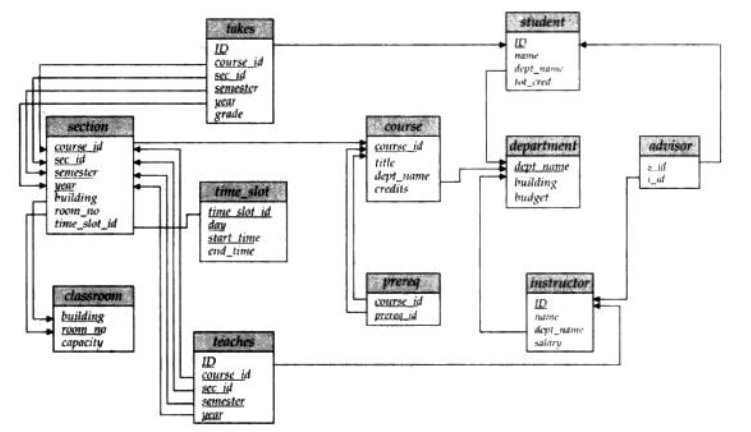
\includegraphics[width=0.8\linewidth]{fig/university_schema_diagram.png}
\end{figure}